\section{Clasificador}

\subsection{Metodología}
\begin{frame}
    \frametitle{Metodología}

    \begin{itemize}
        \item Se utilizan SVM, kNN, DT, GNB y MNB.
        \item Se divide en 80\% entrenamiento y 20\% evaluación.
        \item Se usa validación cruzada sobre el conjunto de entrenamiento para resultados intermedios durante el desarollo y el conjunto de evaluación para el resultado final.
    \end{itemize}
\end{frame}
\note{
    Se usa el conjunto de evaluación al final para no sesgarse demasiado a los resultados.
}

\subsection{Línea base}
\begin{frame}
    \frametitle{Línea base}

    \begin{enumerate}
        \item BoW + MNB

        \item Clasificador que predice según lo que dice la mayoría (Negativo)
    \end{enumerate}

    \begin{center}
        \scriptsize
        \begin{tabular}{ c | r | r | r | r | r | r | r }
            & \multicolumn{1}{c |}{Precisión} & \multicolumn{1}{c |}{Recall} & \multicolumn{1}{c |}{$F_1$} & \multicolumn{1}{c |}{Prec. neg.} & \multicolumn{1}{c |}{Rec. neg.} & \multicolumn{1}{c |}{$F_1$ neg.} & \multicolumn{1}{c}{Acierto} \\
            \hline
            LB1 & \textbf{65,2} & \textbf{82,7} & \textbf{72,9} & \textbf{96,3} & 91,2 & \textbf{93,7} & \textbf{89,7} \\
            \hline
            LB2 & N/A & 0,00 & N/A & 82,5 & \textbf{100,0} & 90,4 & 82,5 \\
        \end{tabular}
    \end{center}
\end{frame}

\subsection{Características}

\begin{frame}
    \frametitle{Características: qué se busca}

    \begin{itemize}
        \item Contradicción y negatividad
        \item Formato e informalidad
        \item Orientación en personas
        \item Temas recurrentes en chistes
    \end{itemize}
\end{frame}

\begin{frame}
    \frametitle{Presencia de animales}

    \begin{itemize}
        \item Se conforma una lista de animales a partir de los chistes de animales de Chistes.com ($DIC_A$)
        \item Intersección de multiconjuntos:
    \end{itemize}

    \begin{center}
        \[
            PresenciaAnimales(tweet) = \frac{|tweet \cap DIC_A|}{\sqrt{|tweet|}}
        \]
    \end{center}
\end{frame}
\note{
    Características simples.
    $tweet$ es visto como una lista de tokens.
    En general todas las featuers se normalizan según el largo del tweet en tokens, para no sesgar.
}

\begin{frame}
    \frametitle{Jerga sexual}

    \begin{itemize}
        \item Se arma un diccionario de jerga sexual mediante \emph{Bootstrapping} en Twitter.
        \item Intersección de multiconjuntos:
    \end{itemize}

    \begin{center}
        \[
            JergaSexual(tweet) = \frac{|tweet \cap DIC_{JS}|}{\sqrt{|tweet|}}
        \]
    \end{center}
\end{frame}

\begin{frame}
    \frametitle{Primera y segunda persona}

    \begin{itemize}
        \item Se busca por palabras flexionadas en primera persona y se hace lo mismo con segunda persona
    \end{itemize}
\end{frame}

\begin{frame}
    \frametitle{Distancia temática}

    \begin{itemize}
        \item Cercanía a un chiste de Chistes.com o cercanía a una oración de la Wikipedia.
        \item BoW + MNB
        \item Categorías
        \begin{itemize}
            \item Chistes cortos
            \item Adivinanzas
            \item Animales
            \item Atlantes
            \item Otros...
        \end{itemize}
    \end{itemize}
\end{frame}
\note{TODO: Aclarar qué es atlantes.}

\begin{frame}
    \frametitle{Diálogo}

    \begin{itemize}
        \item Si el tweet es un diálogo o no
    \end{itemize}
\end{frame}

\begin{frame}
    \frametitle{Preguntas-respuestas}

    \begin{itemize}
        \item Cantidad de preguntas seguidas de respuestas en el tweet.
    \end{itemize}
\end{frame}

\begin{frame}
    \frametitle{Palabras clave}

    \begin{itemize}
        \item Lista de palabras frecuentes en tweets
        \item Intersección de multiconjuntos:
    \end{itemize}

    \begin{center}
        \[
            PalabrasClave(tweet) = \frac{|tweet \cap DIC_{PF}|}{\sqrt{|tweet|}}
        \]
    \end{center}
\end{frame}

\begin{frame}
    \frametitle{Links}

    \begin{itemize}
        \item Cantidad de hipervínculos en el tweet
    \end{itemize}
\end{frame}

\begin{frame}
    \frametitle{Antónimos}

    \begin{itemize}
        \item Cantidad de pares de antónimos en el tweet:
    \end{itemize}

    \begin{center}
        \[
            Antonimos(tweet) = \frac{|\{pares\ de\ antonimos\}|}{\sqrt{|tweet|}}
        \]
    \end{center}
\end{frame}

\begin{frame}
    \frametitle{Hashtags}

    \begin{itemize}
        \item Cantidad de hashtags en el tweet
    \end{itemize}
\end{frame}

\begin{frame}
    \frametitle{Exclamación}

    \begin{itemize}
        \item Cantidad de signos de exclamación:
    \end{itemize}

    \begin{center}
        \[
            Exclamacion(tweet) = \frac{|\{signos\ de\ exclamacion\}|}{\sqrt{|tweet|}}
        \]
    \end{center}
\end{frame}

\begin{frame}
    \frametitle{Palabras mayúsculas}

    \begin{itemize}
        \item Cantidad de palabras totalmente en mayúsculas:
    \end{itemize}

    \begin{center}
        \[
            PalabrasMayusculas(tweet) = \frac{|\{palabras\ mayusculas\}|}{\sqrt{|tweet|}}
        \]
    \end{center}
\end{frame}

\begin{frame}
    \frametitle{Negación}

    \begin{itemize}
        \item Cantidad de ``no'' en el tweet
    \end{itemize}
\end{frame}

\begin{frame}
    \frametitle{Palabras fuera del vocabluario (OOV)}

    \begin{itemize}
        \item Cantidad de palabras fuera del vocabulario, dividiento entre el total
        \item Son varias características:
        \begin{itemize}
            \item Freeling
            \item Freeling-Google
            \item Freeling-Wiktionary
            \item Wiktionary
        \end{itemize}
    \end{itemize}
\end{frame}
\note{
    Las distintas combinaciones de vocabulario debido a costo de uso y debido a ventajas y desventajas de cada uno. \textbf{Freeling} el más barato de usar, offline. Tiene un español más clasico, pero no tiene palabras ``nuevas''. \textbf{Wiktionary} tiene un término medio de todo. Es online, pero no limita su uso. Con \textbf{Google} se pueden obtener muchas palabras ``nuevas'' (como iPhone) y también detección de errores ortográficos, pero limita su uso.
}

\begin{frame}
    \frametitle{Palabras no españolas}

    \begin{itemize}
        \item Cantidad de palabras que tienen caracteres fuera del alfabeto español, normalizado según el total.
    \end{itemize}
\end{frame}

\subsection{Selección de características}
\begin{frame}[allowframebreaks]
    \frametitle{Selección de características}

    \begin{itemize}
        \item ExtraTrees es usado para hacer un ranking de características.
        \item Se utiliza la Eliminación recursiva de atributos para seleccionar aquellos relevantes y no redundantes.
    \end{itemize}

    \framebreak

    ExtraTrees:

    \begin{center}
        \tiny
        \begin{tabular}{ c | r }
            \multicolumn{1}{c |}{\textbf{Característica}} & \multicolumn{1}{c}{\textbf{Valor}} \\
            \hline
            CLASE & 74,05 \\
            \hline
            Diálogo & 10,86 \\
            \hline
            Distancia temática: Otros... & 03,07 \\
            \hline
            Distancia temática: Atlantes & 02,65 \\
            \hline
            Distancia temática: Chistes cortos & 02,53 \\
            \hline
            Preguntas-respuestas & 01,98 \\
            \hline
            Distancia temática: Adivinanzas & 0,95 \\
            \hline
            Distancia temática: Animales & 0,87 \\
            \hline
            Palabras clave & 0,57 \\
            \hline
            Exclamación & 0,57 \\
            \hline
            Hashtags & 0,55 \\
            \hline
            Links & 0,54 \\
            \hline
            Primera persona & 0,21 \\
            \hline
            Segunda persona & 0,15 \\
            \hline
            OOV Freeling & 0,08 \\
            \hline
            Palabras mayúsculas & 0,06 \\
            \hline
            ALEATORIA & 0,06 \\
            \hline
            Jerga sexual & 0,06 \\
            \hline
            Negación & 0,05 \\
            \hline
            OOV Wiktionary & 0,04 \\
            \hline
            OOV Freeling Wiktionary & 0,03 \\
            \hline
            Presencia de animales & 0,03 \\
            \hline
            OOV Freeling Google & 0,03 \\
            \hline
            Antónimos & 0,02 \\
            \hline
            Palabras no españolas & 0,00 \\
        \end{tabular}
    \end{center}

    \framebreak

    Eliminación recursiva de atributos:

    \begin{center}
        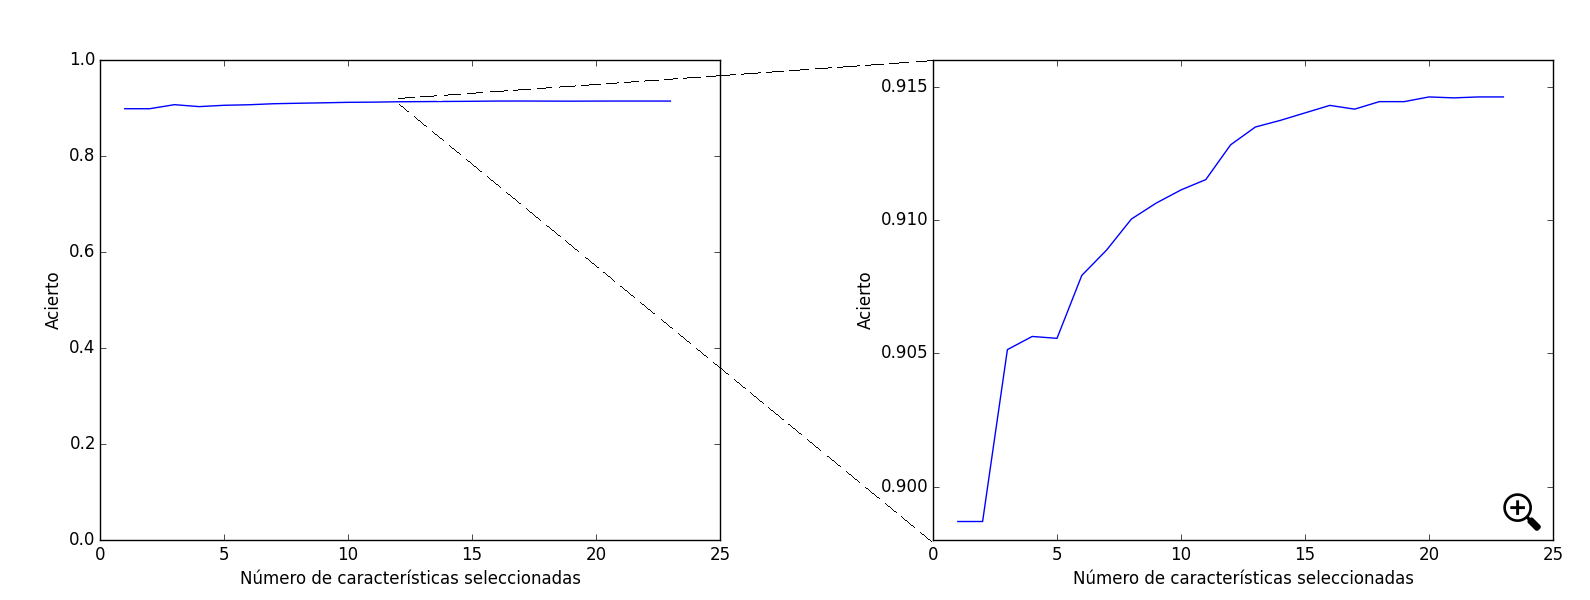
\includegraphics[height=5cm]{rfe.png}

        \vfill

        Se descartan Negación, Palabras no españolas y Antónimos
    \end{center}
\end{frame}

\subsection{Resultados obtenidos}
\begin{frame}
    \frametitle{Resultados obtenidos}

    \begin{center}
        \scriptsize
        \begin{tabular}{ c | r | r | r | r | r | r | r }
            & \multicolumn{1}{c |}{Precisión} & \multicolumn{1}{c |}{Recall} & \multicolumn{1}{c |}{$F_1$} & \multicolumn{1}{c |}{Prec. neg.} & \multicolumn{1}{c |}{Rec. neg.} & \multicolumn{1}{c |}{$F_1$ neg.} & \multicolumn{1}{c}{Acierto} \\
            \hline
            LB1 & \textbf{61,7} & \textbf{84,6} & \textbf{71,4} & \textbf{96,6} & 89,2 & 71,4 & \textbf{88,5} \\
            \hline
            LB2 & N/A & 0,00 & N/A & 83,0 & \textbf{100,0} & \textbf{90,7} & 83,0 \\
            \hline
            \hline
            SVM & 83,6 & 68,9 & \textbf{75,5} & 93,8 & 97,2 & \textbf{95,5} & \textbf{92,5} \\
            \hline
            DT & 66,5 & 67,5 & 67,0 & 93,3 & 93,0 & 93,2 & 88,9 \\
            \hline
            GNB & 57,5 & \textbf{78,2} & 66,3 & \textbf{95,2} & 88,2 & 91,5 & 86,5 \\
            \hline
            MNB & \textbf{84,8} & 60,0 & 70,3 & 92,3 & \textbf{97,8} & 95,0 & 91,4 \\
            \hline
            KNN & 81,3 & 66,3 & 73,0 & 93,4 & 96,9 & 95,1 & 91,7 \\
        \end{tabular}

        \begin{center}
            Mejor técinca: \textbf{SVM}
        \end{center}

        \begin{tabular}{ c | r | r }
            \textbf{son/clasif.} & Positivos & Negativos \\
            \hline
            Positivos & 842 & 381 \\
            \hline
            Negativos & 165 & 5805 \\
        \end{tabular}
    \end{center}
\end{frame}
\note{TODO: decir que es luego del escalado y demás}

\subsection{Otros análisis}

\subsubsection{Evaluación en el conjunto de entrenamiento}
\begin{frame}
    \frametitle{Evaluación en el conjunto de entrenamiento}

    \begin{itemize}
        \item Es una ``cota superior''
    \end{itemize}

    \begin{center}
        \scriptsize
        \begin{tabular}{ c | r | r | r | r | r | r | r }
            & \multicolumn{1}{c |}{Precisión} & \multicolumn{1}{c |}{Recall} & \multicolumn{1}{c |}{$F_1$} & \multicolumn{1}{c |}{Prec. neg.} & \multicolumn{1}{c |}{Rec. neg.} & \multicolumn{1}{c |}{$F_1$ neg.} & \multicolumn{1}{c}{Acierto} \\
            \hline
            SVM & 87,5 & 69,6 & 77,5 & 94,2 & 98,0 & 96,1 & 93,3 \\
            \hline
            DT & \textbf{100,0} & \textbf{98,8} & \textbf{99,4} & \textbf{99,8} & \textbf{100,0} & \textbf{99,9} & \textbf{99,8} \\
            \hline
            GNB & 58,1 & 77,7 & 66,4 & 95,2 & 88,8 & 91,9 & 86,9 \\
            \hline
            MNB & 84,6 & 58,9 & 69,5 & 92,3 & 97,9 & 95,0 & 91,7 \\
            \hline
            KNN & 87,0 & 71,5 & 78,5 & 94,5 & 97,9 & 96,2 & 93,5 \\
        \end{tabular}
    \end{center}
\end{frame}

\begin{frame}
    \frametitle{Evaluación en el conjunto de entrenamiento II}

    \begin{itemize}
        \item ¿Por qué DT no da 100\%? Debería darlo.
        \item Las características no discriminan completamente a la clase.
        \item ¿Hay errores en el corpus?
    \end{itemize}
\end{frame}

\begin{frame}[allowframebreaks]
    \frametitle{Inconsistencias en el corpus}

    \begin{itemize}
        \item Siguiendo la distancia mínima de edición en tweets (la granularidad es una palabra): se encontraron 367 pares de tweets ``parecidos'' pero con distinto valor de la clase objetivo.
    \end{itemize}

    \begin{example}
        Limpiar tu cuarto = 1\% limpieza. 30\% quejarse. 69\% jugar con lo que vas encontrando.
    \end{example}

    \begin{example}
        Limpiar tu cuarto:

        1\% limpieza.

        30\% quejarse.

        69\% jugar con lo que vas encontrando.
    \end{example}

    \note{
        En el primer caso son casi las mismas palabras, pero distinto espaciado y puntuación.
    }

    \framebreak

    \begin{itemize}
        \item Luego se buscan aquellos con mismos valores de atributos pero distinta clase: 30 pares encontrados.
    \end{itemize}

    \begin{example}
        \#TerminarUnaNotaDeSuicidioCon Soy Darks.
    \end{example}

    \begin{example}
        \#SiYoMeLlamaraKevinRoldan Me suicidaria.
    \end{example}
\end{frame}

\begin{frame}
    \frametitle{Inconsistencias en el corpus III}

    \begin{itemize}
        \item Hay inconsistencias en la anotación (era esperado)
        \item Hay una mejora sobre el corpus de entrenamiento, en la ``cota superior'', quitando estas instancias:

        \begin{center}
            \scriptsize
            \begin{tabular}{ c | r | r | r | r | r | r | r }
                \textbf{SVM} & \multicolumn{1}{c |}{Precisión} & \multicolumn{1}{c |}{Recall} & \multicolumn{1}{c |}{$F_1$} & \multicolumn{1}{c |}{Prec. neg.} & \multicolumn{1}{c |}{Rec. neg.} & \multicolumn{1}{c |}{$F_1$ neg.} & \multicolumn{1}{c}{Acierto} \\
                \hline
                Antes & 87,5 & 69,6 & 77,5 & 94,2 & 98,0 & 96,1 & 93,3 \\
                \hline
                Después & \textbf{89,0} & \textbf{71,3} & \textbf{79,1} & \textbf{94,7} & \textbf{98,3} & \textbf{96,5} & \textbf{94,0} \\
            \end{tabular}
        \end{center}
    \end{itemize}

    \begin{itemize}
        \item Y en el de corpus de evaluación:

        \begin{center}
            \scriptsize
            \begin{tabular}{ c | r | r | r | r | r | r | r }
                \textbf{SVM} & \multicolumn{1}{c |}{Precisión} & \multicolumn{1}{c |}{Recall} & \multicolumn{1}{c |}{$F_1$} & \multicolumn{1}{c |}{Prec. neg.} & \multicolumn{1}{c |}{Rec. neg.} & \multicolumn{1}{c |}{$F_1$ neg.} & \multicolumn{1}{c}{Acierto} \\
                \hline
                Antes & 83,6 & 68,9 & 75,5 & 93,8 & 97,2 & 95,5 & 92,5 \\
                \hline
                Después & \textbf{85,7} & \textbf{69,2} & \textbf{76,6} & \textbf{94,2} & \textbf{97,8} & \textbf{95,9} & \textbf{93,1} \\
            \end{tabular}
        \end{center}
    \end{itemize}
\end{frame}

\subsubsection{Tweets censurados}
\begin{frame}
    \frametitle{Tweets censurados}

    \begin{itemize}
        \item El clasificador está sesgado a no conocer los tweets con contenido explícito
        \item Se anotan a mano los 303 tweets censurados y se agregan
        \item Hay una pequeña mejora:
        \begin{center}
            \scriptsize
            \begin{tabular}{ c | r | r | r | r | r | r | r }
                \textbf{SVM} & \multicolumn{1}{c |}{Precisión} & \multicolumn{1}{c |}{Recall} & \multicolumn{1}{c |}{$F_1$} & \multicolumn{1}{c |}{Prec. neg.} & \multicolumn{1}{c |}{Rec. neg.} & \multicolumn{1}{c |}{$F_1$ neg.} & \multicolumn{1}{c}{Acierto} \\
                \hline
                Antes & 83,6 & 68,9 & 75,5 & \textbf{93,8} & \textbf{97,2} & \textbf{95,5} & \textbf{92,5} \\
                \hline
                Después & \textbf{84,0} & \textbf{69,6} & \textbf{76,1} & 93,7 & 97,2 & 95,4 & 92,3 \\
            \end{tabular}
        \end{center}
        \item Un nuevo estudio de importancia de las características revela que no varía Jerga sexual: se agrega más variedad que jerga sexual.
    \end{itemize}
\end{frame}

\subsubsection{Restricción a cuentas humorísticas}
\begin{frame}
    \frametitle{Restricción a cuentas humorísticas}

    \begin{itemize}
        \item Es una tarea más difícil
        \item Igualmente se logran buenos resultados:

        \begin{center}
            \scriptsize
            \begin{tabular}{ c | r | r | r | r | r | r | r }
                & \multicolumn{1}{c |}{Precisión} & \multicolumn{1}{c |}{Recall} & \multicolumn{1}{c |}{$F_1$} & \multicolumn{1}{c |}{Prec. neg.} & \multicolumn{1}{c |}{Rec. neg.} & \multicolumn{1}{c |}{$F_1$ neg.} & \multicolumn{1}{c}{Acierto} \\
                \hline
                SVM & \textbf{81,9} & 73,8 & 77,6 & 78,5 & \textbf{85,4} & \textbf{81,8} & \textbf{79,9} \\
                \hline
                DT & 74,5 & 75,5 & 75,0 & 72,2 & 71,1 & 71,7 & 74,1 \\
                \hline
                GNB & 78,7 & 78,6 & \textbf{78,6} & 76,1 & 76,3 & 76,2 & 77,5 \\
                \hline
                MNB & 68,5 & \textbf{85,5} & 76,1 & \textbf{83,3} & 64,6 & 72,9 & 74,6 \\
                \hline
                KNN & 79,2 & 73,0 & 76,0 & 77,4 & 82,9 & 80,1 & 78,1 \\
            \end{tabular}
        \end{center}
    \end{itemize}
\end{frame}

\begin{frame}
    \frametitle{Métricas ponderadas según calificación}

    \begin{itemize}
        \item Tiene sentido sólo para los tweets que tuvieron votos y para la medida recall
        \item Promedio de estrellas, $PE_t = \frac{\sum_{i = 1}^{5} i \times v_{ti}}{v_t}$
        \item $recall_{ponderado} = \frac{\sum_{t \in VP} PE_t} {\sum_{t \in VP} PE_t + \sum_{t \in FN} PE_t} = 70.68\%$
        \item $\frac{recall_{ponderado}}{recall} = \frac{prom_{VP}}{prom_H} = 1.0266$
        \item Hay un (muy) leve sesgo del clasificador SVM a dar como positivos aquellos tweets que tienen mayor promedio de estrellas.
        \item Matriz de confusión:

        \begin{center}
            \begin{tabular}{ c | r | r }
                \textbf{son/clasificados} & Humor & No humor \\
                \hline
                Humor & 2,7227 & 2,4961 \\
                \hline
                No humor & 0,0256 & 0,0300 \\
            \end{tabular}
        \end{center}
    \end{itemize}
\end{frame}

\subsubsection{Clasificación según categorías de cuentas no humorísticas}
\begin{frame}
    \frametitle{Clasificación según categorías de cuentas no humorísticas}

    \begin{center}
        \scriptsize
        \begin{tabular}{ c | r | r | r | r | r | r | r }
            \textbf{SVM} & \multicolumn{1}{c |}{Precisión} & \multicolumn{1}{c |}{Recall} & \multicolumn{1}{c |}{$F_1$} & \multicolumn{1}{c |}{Prec. neg.} & \multicolumn{1}{c |}{Rec. neg.} & \multicolumn{1}{c |}{$F_1$ neg.} & \multicolumn{1}{c}{Acierto} \\
            \hline
            Noticias & \textbf{97,0} & \textbf{95,2} & \textbf{96,1} & \textbf{97,0} & \textbf{98,1} & \textbf{97,5} & \textbf{97,0} \\
            \hline
            Reflexiones & 95,0 & 83,0 & 88,6 & 84,0 & 95,3 & 89,3 & 88,9 \\
            \hline
            Curiosidades & 94,6 & 83,7 & 88,9 & 88,2 & 96,3 & 92,1 & 90,7 \\
        \end{tabular}
    \end{center}
\end{frame}
